\documentclass[12pt,titlepage]{article}
\usepackage[linktoc=all]{hyperref}
\usepackage{listings}
\usepackage{graphicx}
\usepackage{xcolor}

% Define style for source code
\lstdefinestyle{cppstyle}{
  belowcaptionskip=1\baselineskip,
  breaklines=true,
  language=C++,
  showstringspaces=false,
  numbers=left,
  basicstyle=\footnotesize\ttfamily,
  keywordstyle=\bfseries\color{green!40!black},
  commentstyle=\itshape\color{purple!40!black},
  identifierstyle=\color{blue},
  stringstyle=\color{orange},
}
\lstset{escapechar=@, style=cppstyle}

\begin{document}
\title{ECE 303 Lab Technical Memos}
\author{Nicholas Sica}
\date{October 2, 2020}
\maketitle

\tableofcontents
\newpage

\section{Week 1 Lab}
\subsection{Discussion}
The point of this lab was to introduce us to the Arduino toolkit and allow anyone who is new to the platform time to adjust and get familiar with the tools presented to them. The lab was straightforward, connect an LED and resistor to a pin on the arduino and writing simplistic code to change the pulse width modulation values. The output is as expected, with the intensity of the light changing based off the number put into the serial monitor, zero being off and 255 being full brightness.
\begin{figure}[!htb]
  \centering
  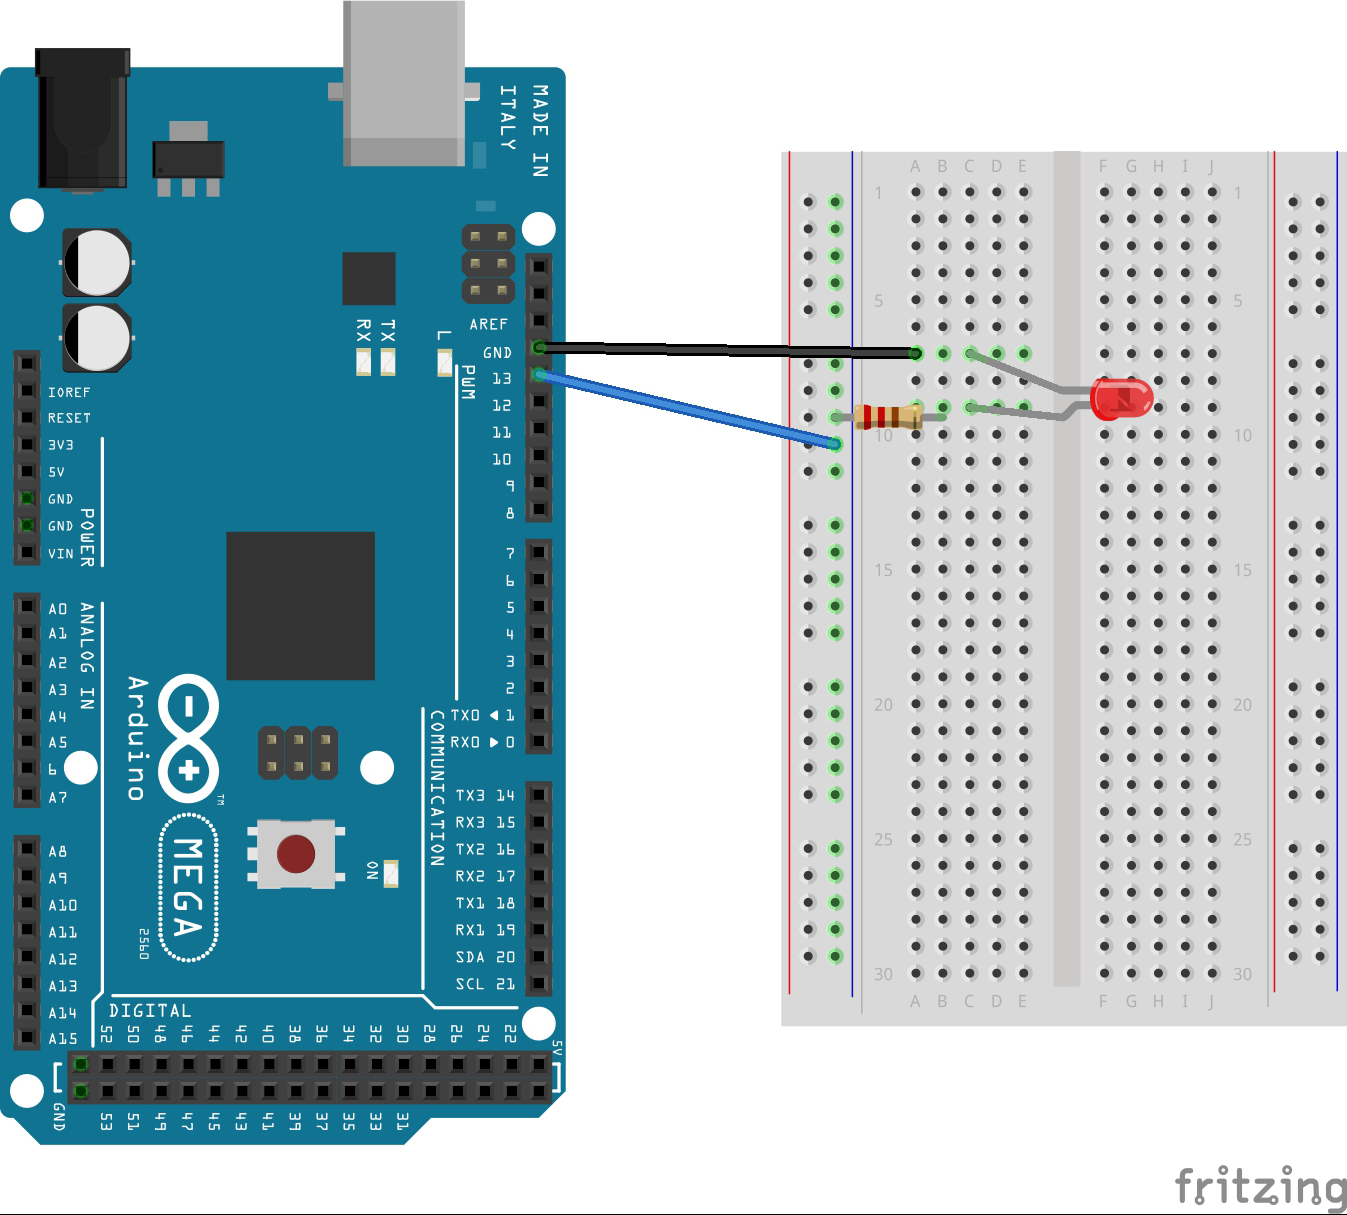
\includegraphics[width=5.0in]{figure_1_1.png}
  \caption{Basic LED Circuit Setup}\label{fig:lab_2}
\end{figure}
\subsection{Software}
\begin{minipage}{\linewidth}
  \lstinputlisting[caption={Lab 2 Code}, captionpos=b, label={lst:lab_2},
language=C++]{../lab_2/src/main.cpp}
\end{minipage}
\newpage
\section{Week 2 Lab}
\subsection{Discussion}
This lab was used to get us acquainted with timers and learn not only how to set up the correct bit values, but also how to use them efficiently. A lot of the time was spent debugging the bit values that the different masks are initialized with as well as learning how to turn the interrupts off efficiently. When run, every LED blinks at a slow pace and each guess for the code either causes it to blink faster, if wrong, or turn off, if correct. When the user is out of attempts, the remaining LEDs stay permanently on.
\begin{equation} \label{eq:ocr3a}
  OCR3A = \frac{16\times10^6}{p\times f} - 1
\end{equation}
The value of the register was found using equation~\ref{eq:ocr3a}, where p is the prescalar, in this case 1024, and f is the target frequency, in this case around 0.5 hertz or a 2 second period. Every subsequent wrong guess, it was divided by two to make it go faster.
\begin{figure}[!htb]
  \centering
  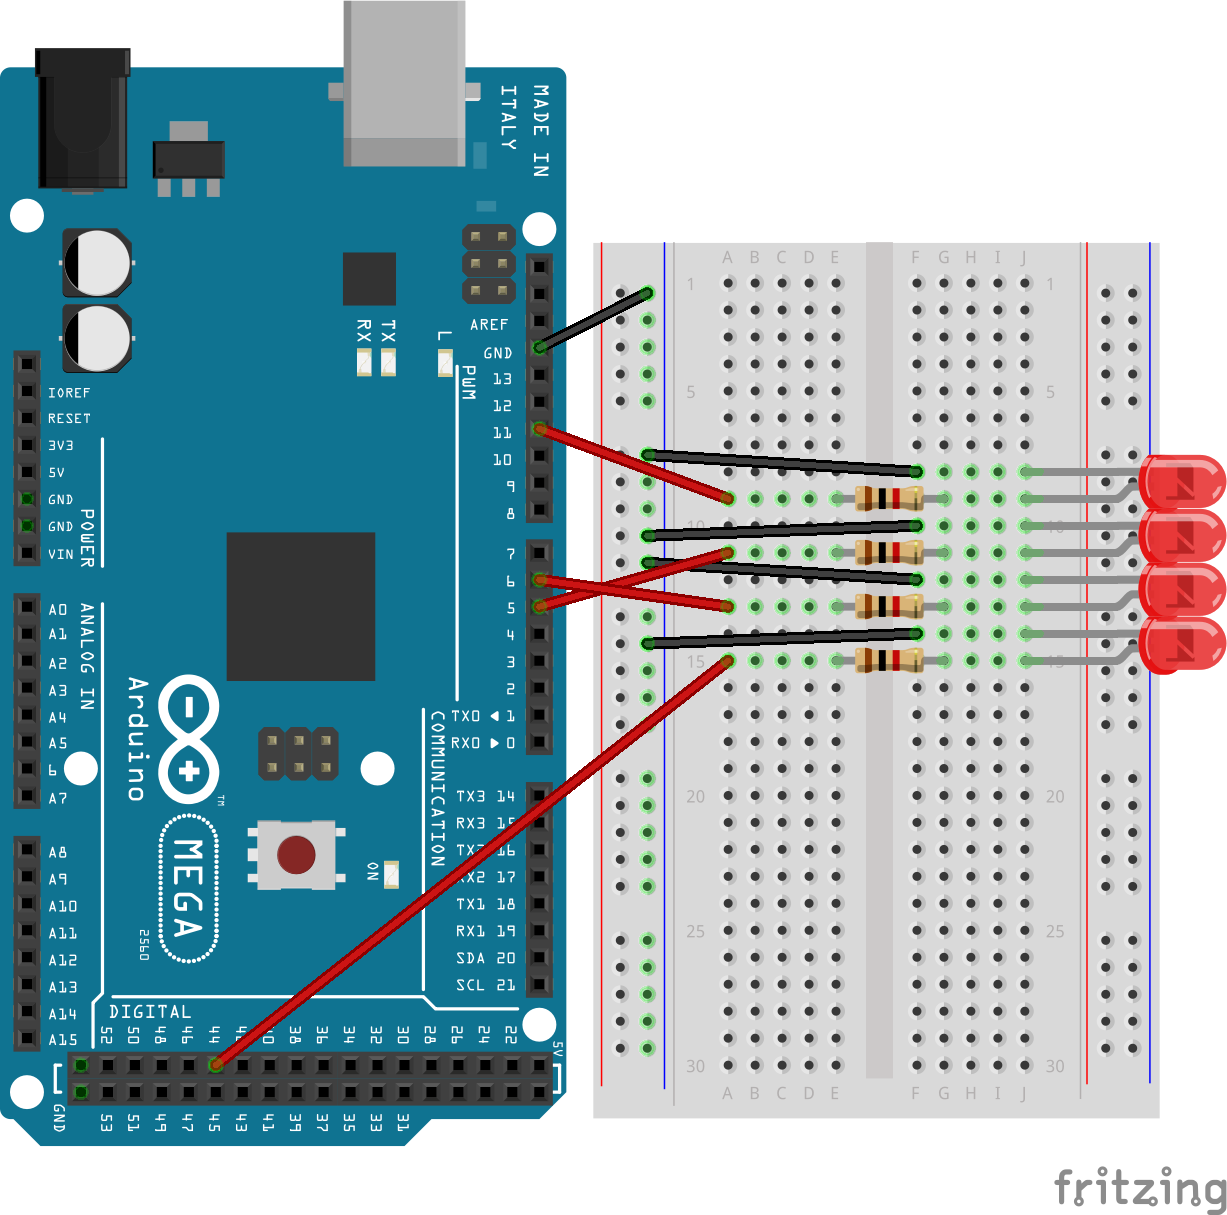
\includegraphics[width=3.25in]{lab_3_schematic.png}
  \caption{Codebreaker Circuit Setup}\label{fig:lab_3}
\end{figure}
\subsection{Hardware}
Figure~\ref{fig:lab_3} shows the setup of the circuit. The setup of the hardware was very similar to the previous lab, but this time there are four LEDs and care was taken to connect to them to the correct pin corresponding to the timer we want to use for it.
\subsection{Software}
  \lstinputlisting[caption={Lab 3 Code}, captionpos=b label={lst:lab_3}, language=C++]{../lab_3/src/main.cpp}
\end{document}

%%% Local Variables:
%%% mode: latex
%%% TeX-master: t
%%% End:
